\documentclass[11pt]{article}

\usepackage[T1]{fontenc}
\usepackage[utf8]{inputenc}
\usepackage{lmodern}
\usepackage[english]{babel}

\usepackage[margin=1in]{geometry}
\usepackage{amsmath,amssymb,amsthm}
\usepackage{booktabs}
\usepackage[expansion=false]{microtype}
\usepackage{enumitem}
\usepackage{pgfplots}
\pgfplotsset{compat=1.18}
\usepackage[colorlinks=true,allcolors=blue]{hyperref}
\usepackage{listings}
\lstset{basicstyle=\ttfamily\scriptsize,breaklines=true,columns=fullflexible,
  keepspaces=true,showstringspaces=false,frame=single,framesep=3pt,
  xleftmargin=4pt,xrightmargin=2pt,aboveskip=4pt,belowskip=2pt}
\setlength{\emergencystretch}{3em}

\newtheorem{theorem}{Theorem}
\newtheorem{lemma}{Lemma}
\newtheorem{corollary}{Corollary}
\newtheorem{proposition}{Proposition}
\newtheorem{assumption}{Assumption}
\theoremstyle{remark}
\newtheorem{remark}{Remark}

\newcommand{\lst}{\lambda_{\mathrm{st}}}
\newcommand{\lred}{\lambda_{\mathrm{red}}}
\newcommand{\lirr}{\lambda_{\mathrm{irr}}}
\newcommand{\Padv}{P_{\mathrm{adv}}}
\newcommand{\eseg}{\varepsilon_{\mathrm{seg}}}
\newcommand{\am}{\bar\alpha_m}
\newcommand{\bm}{\bar\beta_m}
\newcommand{\Hraw}{H_{\mathrm{raw}}}
\newcommand{\Hgated}{H_{\mathrm{gated}}}
\newcommand\blfootnote[1]{\begingroup\renewcommand\thefootnote{}\footnote{#1}\addtocounter{footnote}{-1}\endgroup}

\title{\vspace{-2em}A Fault-Tolerance Threshold for Gated Agentic Computation:\\
\large Reliable Long-Horizon Work from Unreliable Executors}

\author{Ivo Matijašević\\ \small Independent Researcher \\ \small ivomatijasevic@gmail.com}
\date{June 2026}

\begin{document}
\maketitle
\blfootnote{\textcopyright~2026 Ivo Matijašević.\ This work is licensed under a Creative Commons
Attribution 4.0 International (CC BY 4.0) license, \url{https://creativecommons.org/licenses/by/4.0/}.}

\begin{abstract}
Autonomous agents (whether language-model based, human, or hybrid) commit errors at an
approximately constant rate per unit of work---a constant-hazard baseline we adopt, motivated by
reported time-horizon fits rather than claimed as a universal law---so the probability that a long
task completes without fault decays exponentially in its length.
The task length at which an agent succeeds
half the time---its \emph{horizon}---has become a leading proposed metric of agentic capability, and
empirically it has grown exponentially over recent years.
We ask a different question: given a
fixed agent, how far can \emph{verification} extend its reliable horizon?
We model long-horizon
work as a sequence of checkpointed segments, each verified by a stack of imperfect gates combined
by majority vote, and we prove a fault-tolerance threshold analogous to von Neumann's
reliable-computation-from-unreliable-components result and to the quantum threshold theorem.
\textbf{(i)} When gates are conditionally independent and better than chance, a stack of
$O(\log T)$ gates per checkpoint achieves any target reliability over horizon $T$, yielding a
multiplicative time overhead that is likewise $O(\log T)$.
\textbf{(ii)} When gates share a blind spot---a stealth mass
$\lst$ of faults invisible to the entire gate family---the reliable horizon is capped at
$\Hgated \approx \Hraw/\lst$ regardless of gate count.
\textbf{(iii)} The cost-optimal checkpoint
interval is $s^\star \approx \sqrt{G/\lambda}$, a direct analogue of the Young--Daly checkpoint
formula with verification cost in place of crash-recovery cost.
The binding constraint on
autonomous horizon is therefore not raw model capability but the diversity of the verification
stack, a quantity partly estimable from a system's own telemetry and targeted audits.
We further decompose the stealth mass
into a diversity-reducible part and a specification-bound irreducible floor, and we note that a
recent large-scale $N$-version experiment with coding agents motivates the bounded regime~(ii) for
realistic systems.
We numerically illustrate all three results in simulation and specify a falsifiable
experiment on agentic task suites.
\end{abstract}

\section{Introduction}
A coding agent that completes a single function correctly $95\%$ of the time will complete a
$100$-step project correctly with probability $0.95^{100}\approx 0.6\%$.
This multiplicative
decay---not any single hard step---is the fundamental obstacle to long-horizon autonomy.
The
quantity that has emerged to measure progress against it is the \emph{horizon}: the task length,
in human-equivalent time, at which an agent succeeds with probability one half.
Measurements of
frontier systems report that this horizon has roughly doubled on a fixed cadence over several
years~\cite{metr2025}, and an analysis of the same data finds it consistent with a constant
per-unit hazard---an exponential, ``half-life'' decay of success in task duration~\cite{ord2025}.
The prevailing reading of this trend is that horizon is a property of model capability, to be
extended by training better models.
We argue, and prove within a standard model, that this is only
half the story.
Errors that compound can also be \emph{intercepted}: if work is divided into
verifiable segments and each segment is checked before the agent proceeds, then detected faults
are repaired locally and never compound.
The reliability of the whole is then governed by the
quality of the checking, not directly by the quality of the agent.
This is precisely the logic by
which von Neumann obtained reliable computation from unreliable components~\cite{vonneumann1956},
by which fault-tolerant quantum computation became possible below a noise
threshold~\cite{aharonov1997}, and by which classical software is shipped at all.
While contemporary empirical studies---such as Ron et al.~\cite{ron2026}---confirm that AI
coding agents suffer from significant common-mode failures when generating code for static
specifications, a formal model mapping these vulnerabilities to long-horizon sequential
execution has been missing.
We bridge this gap, establishing the universal mathematical
boundaries of verification stacks over arbitrary horizons~$T$ and making them quantitative for
agentic work. Our contributions:
\begin{itemize}[leftmargin=1.4em,itemsep=2pt]
\item \textbf{A threshold theorem (Thm.~\ref{thm:threshold}):} below a gate-error threshold,
reliable work of unbounded horizon is achievable at overhead logarithmic in horizon;
above it,
horizon is bounded.
\item \textbf{A ceiling theorem (Thm.~\ref{thm:ceiling}):} with correlated gate blind spots of
mass $\lst$, horizon is capped at $\approx \Hraw/\lst$, making verification diversity the binding
constraint.
\item \textbf{A stealth decomposition (Prop.~\ref{prop:decomp}):} $\lst=\lred+\lirr$ separates the
mass that diversity can remove from a specification-bound floor that it cannot, identifying
\emph{where} diversity stops paying.
\item \textbf{An optimal-interval result (Thm.~\ref{thm:interval}):} the cost-minimizing
checkpoint spacing is $s^\star\approx\sqrt{G/\lambda}$, a direct analogue of Young--Daly
checkpointing~\cite{young1974,daly2006}.
\item Numerical simulations checking the model predictions, and a specified experiment (\S\ref{sec:experiment})
whose outcome would confirm or falsify the central claim.
\end{itemize}

\section{Model}
An agent performs work parameterized by a continuous duration. Faults arrive as a homogeneous
Poisson process of rate $\lambda$;
thus a stretch of work of length $t$ is fault-free with
probability $e^{-\lambda t}$, and the ungated horizon (the $t$ at which success probability is
$\tfrac12$) is $H_0=\ln 2/\lambda$.
The constant-hazard assumption is an idealization, adopted
because it fits reported agentic data~\cite{ord2025} and because it isolates the phenomenon of
interest;
\S\ref{sec:limitations} discusses its failure modes.

\paragraph{Checkpointing.} Work is divided into segments of length $s$.
After each segment a gate
stack renders a verdict; on fail the segment is rolled back and recomputed, on pass the agent
advances.
A segment is \emph{bad} if it contains at least one fault, which occurs with probability
$p=1-e^{-\lambda s}$.
\paragraph{Gates.} A gate is a binary test on a segment with two error rates:
the false-accept rate $\alpha=\Pr[\text{pass}\mid\text{bad}]$ and the false-reject rate
$\beta=\Pr[\text{fail}\mid\text{good}]$.
A stack of $m$ gates is combined by majority vote,
yielding effective rates $(\am,\bm)$.
We write a \emph{family} for a set of gates whose errors are
statistically dependent (e.g.\ sharing a base model or a test modality).
\paragraph{Stealth mass.} The key correlation parameter is the stealth mass $\lst\in[0,1]$: the
fraction of bad segments that pass every gate in a family with probability one.
These are faults
the entire family is blind to. We adopt the \emph{stealth mixture}: a bad segment is stealthy with
probability $\lst$ (and then passes regardless of $m$), and otherwise each gate independently
false-accepts with probability $\alpha'$.
Here $\alpha'$ is the per-gate false-accept rate
\emph{conditional} on the segment not being stealthy; a single gate's unconditional
accept-given-bad rate is then $\lst+(1-\lst)\alpha'$, and the two coincide ($\alpha=\alpha'$) in the
independence regime $\lst=0$ of Thm.~\ref{thm:threshold}.
The simulation (\S\ref{sec:simulation})
fixes this conditional rate at $\alpha'=0.3$, reported there as $\alpha$.
\paragraph{The stealthy regime is the realistic one.} The independence idealization $\lst=0$
underlying Thm.~\ref{thm:threshold} is empirically the exception, not the rule.
This was first
established for human-written multiversion software by Knight and Leveson~\cite{knight1986}, whose
independently developed implementations exhibited coincident failures far in excess of the
independence prediction, with a small number of fault families dominating~\cite{brilliant1990};
the theoretical inevitability of such correlation was argued by Eckhardt and Lee~\cite{eckhardt1985}
and Littlewood and Miller~\cite{littlewood1989}.
The phenomenon persists, undiminished, for modern
AI coding agents: in a faithful reproduction of the Knight--Leveson experiment across five agent
systems, twenty-three models, and three languages, Ron et al.~\cite{ron2026} observe $429$
coincident-failure inputs where independence predicts $115.4$ ($z=29.2$), with the dominant
shared fault---computing a circumcircle in place of a minimum enclosing circle---appearing across
\emph{every} agent and language boundary.
A blind spot common to the entire generator population
is exactly a nonzero $\lst$.
This motivates treating realistic gate stacks as operating in the bounded regime of
Thm.~\ref{thm:ceiling}, which is why its decomposition (Prop.~\ref{prop:decomp}) is the operative
result.
\begin{assumption}[Checkpoint completeness]\label{a1}
A genuinely good, passed segment screens off the past: downstream success is conditionally
independent of how the segment was produced.
Goodhart faults---work satisfying the checkable contract but violating intent (i.e., when optimizing for a proxy metric degrades the true goal)---are not excluded by this assumption; they are accounted as part of $\lst$ (\S\ref{sec:limitations}).
\end{assumption}
\begin{assumption}[Memoryless retries and segments]\label{a2}
Fault arrivals are independent across recomputation rounds and across segments.
Realizing this
requires that a rollback restores a clean context, not merely a clean artifact
(\S\ref{sec:design}).
\end{assumption}
\begin{assumption}[Conditional gate independence]\label{a3}
Outside the stealth event, gate errors are mutually independent given the segment's true status.
\end{assumption}

\section{Results}

\begin{lemma}[Per-segment slip]\label{lem:slip}
Under Assumptions~\ref{a1}--\ref{a3}, the recomputation loop for a segment advances in a given
round with probability $\Padv=(1-p)(1-\bm)+p\,\am$, and the advanced segment is bad (a \emph{slip})
with probability
\[
\eseg=\frac{p\,\am}{\Padv}.
\]
\end{lemma}
\begin{proof}
Rounds are i.i.d.\ by Assumption~\ref{a2}. Conditioning on the round that advances, the posterior
probability of badness is given by Bayes' rule with prior $p$ and likelihoods $\am$ (bad passes)
and $1-\bm$ (good passes);
normalizing yields the claim.
\end{proof}

\noindent Over $n=T/s$ independent segments, end-to-end success is $(1-\eseg)^n$.
\begin{theorem}[Threshold and logarithmic overhead]\label{thm:threshold}
Suppose $\lst=0$ and each gate satisfies $\alpha<\tfrac12$ and $\beta<\tfrac12$ with conditional
independence (Assumption~\ref{a3}).
Then for every horizon $T$ and target error $\varepsilon$, a
majority stack of
\[
m=O\!\left(\log\frac{T}{\varepsilon s}\right)
\]
gates per checkpoint achieves end-to-end success at least $1-\varepsilon$, at total expected time
at most $T\cdot O\!\big(1+(g/s)\,m\big)$ where $g$ is the per-gate time---i.e.\ multiplicative
overhead $O(\log T)$.
Conversely, if the effective majority accuracy on bad segments is at most
$\tfrac12$, no $m$ achieves unbounded horizon.
\end{theorem}
\begin{proof}
By Hoeffding's inequality applied to the majority vote of $m$ independent tests,
$\am\le\exp(-2m(\tfrac12-\alpha)^2)$ and $\bm\le\exp(-2m(\tfrac12-\beta)^2)$, both decaying
exponentially in $m$.
Choose $m$ so that $\am\le\varepsilon s(1-p)/(2Tp)$ and $\bm\le\tfrac12$;
the first requirement dominates and is met for $m=O(\log(Tp/\varepsilon s))$ with constant
$1/(2(\tfrac12-\alpha)^2)$.
Then by Lemma~\ref{lem:slip},
$\eseg\le p\am/[(1-p)(1-\bm)]\le\varepsilon s/T$, and a union bound over $n=T/s$ segments gives
total error at most $\varepsilon$.
The expected time per advanced segment is
$(s+mg)/\Padv\le 2(s+mg)/(1-p)$ once $\bm\le\tfrac12$; summing over $n$ segments gives the stated
overhead.
For the converse, majority accuracy at most $\tfrac12$ on bad segments leaves $\am$
bounded away from $0$, so $\eseg\ge c\,p>0$ and success decays geometrically in $n$.
\end{proof}

\begin{remark}\label{rem:threshold}
The condition $\max(\alpha,\beta)<\tfrac12$ is simultaneously von Neumann's component-error
threshold, Condorcet's juror-competence condition~\cite{condorcet1785}, and the shape of the
quantum threshold theorem~\cite{aharonov1997}.
The cost in gates per decade of horizon is
$\approx\ln 10/(2\gamma^2)$ with edge $\gamma=\tfrac12-\alpha$;
weak gates ($\gamma=0.2$) cost
four times as much per decade as strong ones ($\gamma=0.4$). Edge, squared,
dominates.
\end{remark}

\begin{theorem}[Horizon ceiling]\label{thm:ceiling}
If the gate family has stealth mass $\lst>0$, then for every $m$,
\[
\mathrm{success}(T)\le(1-p\,\lst)^{T/s},
\qquad\text{hence}\qquad
\Hgated\le\frac{s\ln 2}{p\,\lst}=\frac{\ln 2}{\lambda\,\lst}\,\big(1+O(\lambda s)\big).
\]
That is, gating multiplies the reliable horizon by at most $1/\lst$.
\end{theorem}
\begin{proof}
Stealthy bad segments pass unanimously, so $\am\ge\lst$ for all $m$. By Lemma~\ref{lem:slip},
$\eseg\ge p\lst$ (using $\Padv\le 1$), whence the success bound;
solving for the half-success
horizon and using $p=1-e^{-\lambda s}\ge\lambda s(1-\lambda s/2)$ gives the rest.
\end{proof}

\noindent The bound is the $\am\to\lst$, $\Padv\to1$ limit. In any realization it is strict: the
within-family residual leaves $\am>\lst$ and recomputation makes $\Padv<1$, so by
Lemma~\ref{lem:slip} $\eseg>p\lst$ and the realized horizon multiplier sits strictly below
$1/\lst$ (Fig.~\ref{fig:val}b).

\begin{corollary}[Diversity multiplies the ceiling]\label{cor:diversity}
For two families with \emph{independent} stealth events of masses $\lst^{(1)},\lst^{(2)}$,
requiring a segment to pass both families gives combined stealth mass $\lst^{(1)}\lst^{(2)}$.
Depth
within a family cannot reduce $\lst$; diversity across families multiplies it down.
\end{corollary}

\begin{proposition}[Stealth decomposition]\label{prop:decomp}
Model the stealth event of a bad segment as a two-component mixture (a modeling choice; richer
correlation structures interpolate between its two extremes): with probability $\lirr$ it is
\emph{irreducibly} stealthy---a blind spot common to every family; otherwise, independently for
each family, it is \emph{reducibly} stealthy to that family with conditional probability $\rho$.
A single family's stealth mass is then $\lst=\lirr+(1-\lirr)\rho$, with reducible part
$\lred=(1-\lirr)\rho$.
Requiring a segment to pass $k$ independent families leaves the irreducible
part intact and drives the reducible part as $\rho^{k}$, so
\[
\lst^{(1:k)}=\lirr+(1-\lirr)\rho^{k}\;\xrightarrow[k\to\infty]{}\;\lirr,
\]
and hence, for any diversity breadth or depth, the gated horizon is bounded by
\[
\Hgated\;\le\;\frac{\Hraw}{\lirr}.
\]
\end{proposition}
\begin{proof}
A segment is stealthy to all $k$ families iff it is irreducibly stealthy (probability $\lirr$) or,
failing that, reducibly stealthy to each of the $k$ families independently (probability
$(1-\lirr)\rho^{k}$, as in Corollary~\ref{cor:diversity}).
Summing gives
$\lst^{(1:k)}=\lirr+(1-\lirr)\rho^{k}\ge\lirr$, and substituting into Theorem~\ref{thm:ceiling}
gives the horizon bound.
\end{proof}

\begin{remark}[What the two terms are]\label{rem:decomp}
$\lirr$ is the specification/intent floor: faults that satisfy the checkable contract but violate
the goal (\S\ref{sec:limitations}), or that arise where the shared specification is itself
ambiguous, trap \emph{every} family regardless of lineage and are invisible to diversity.
Only
reality grounding---execution against the true environment, or specification refinement---lowers
$\lirr$. $\lred$ is the lineage-correlated mass;
it is bounded by the representation divergence
between families and is the only mass that diversity removes.
The decomposition is visible in the
agentic data of Ron et al.~\cite{ron2026}: the circumcircle fault crosses every agent and language
boundary---a shared blind spot of the entire studied population (a large $\lst$) whose
classification depends on the verifier, since an execution-grounded oracle would catch it
($\lred$) while a checker derived from the same specification would not---whereas a
tolerance-induced angle ambiguity that splits only certain model lineages is a clear $\lred$
contribution.
Majority voting helping on average---their mean
failure count falls from $387.4$ to $131.0$ for three-version units---while a hard core of
co-failures survives is precisely diversity consuming $\lred$ and flooring at $\lirr$.
\end{remark}

\begin{theorem}[Optimal checkpoint interval]\label{thm:interval}
Let $G=mg$ be the per-checkpoint verification time. The time per unit of useful work,
$C(s)\approx\dfrac{(1+G/s)\,e^{\lambda s}}{1-\bm}$, is minimized at $s^\star\approx\sqrt{G/\lambda}$,
with minimal overhead $\approx 1+2\sqrt{G\lambda}$.
\end{theorem}
\begin{proof}
$\ln C(s)=\ln(1+G/s)+\lambda s+\text{const}$. Differentiating, the first-order condition is
$G/(s(s+G))=\lambda$, i.e.\ $s(s+G)=G/\lambda$; for $s\gg G$ (equivalently $G\lambda\ll1$) the
solution is $s^\star=\sqrt{G/\lambda}\,(1+o(1))$.
\end{proof}
\begin{remark}\label{rem:youngdaly}
This is the Young--Daly optimal-checkpoint-interval result~\cite{young1974,daly2006} with
verification cost replacing crash-recovery cost.
Four decades of checkpoint--restart engineering
thus transfer to agent design: checkpoint more often when the agent is weak (high $\lambda$) or
gates are cheap (low $G$).
\end{remark}

\section{Simulation}\label{sec:simulation}
We numerically check the results in a discrete-event simulation of the model (parameters $\alpha=0.3$,
$\beta=0.1$, $\lambda=1$, $s=0.25$, per-gate cost $g=0.05$ unless varied).
These give $\lambda s=0.25$ (segment-badness $p\approx0.221$)---deliberately a \emph{moderate}-$p$
regime, not the small-$p$ limit. Because every experiment evaluates the exact closed forms rather
than their small-$p$ expansions, the $O(\lambda s)$ corrections (of order $10\%$ here) to the
$1+O(\lambda s)$ of Thm.~\ref{thm:ceiling} and the $s\gg G$ of Thm.~\ref{thm:interval} are included
exactly, so the reported numbers are not small-$p$ approximations.
The full,
self-contained script is reproduced in Appendix~\ref{app:code} and is also available at
\url{https://github.com/ivmat/gated-computation-sim}.

\paragraph{Per-segment slip (Lemma~\ref{lem:slip}).} For a representative stack ($m=5$), predicted
$\eseg=0.0446$ versus Monte-Carlo $0.0428$ over $2\times10^4$ trials.
\paragraph{Threshold regime (Thm.~\ref{thm:threshold}).} With $\lst=0$, the gate count required
for $90\%$ end-to-end success grows linearly in $\log T$ (Fig.~\ref{fig:val}a), confirming
logarithmic overhead.
The per-gate cost $g$ is an \emph{arbitrary} illustrative constant
(we have no empirical value for it): it enters the result only through the ratio $g/s$, which
sets the vertical scale of the overhead via $\text{overhead}=(1+(g/s)\,m)/\Padv$ (the $1/\Padv$
factor is the expected recomputation count of rejected segments; Lemma~\ref{lem:slip}), and leaves
both the required gate counts and the per-decade slope of Remark~\ref{rem:threshold} unchanged.
We fix
$g=0.05$, i.e.\ $g/s=0.2$.
\paragraph{Ceiling (Thm.~\ref{thm:ceiling}).} With $m=21$ fixed, the horizon multiplier over the
ungated baseline grows as $\lst$ shrinks ($4.1\times$ at $\lst=0.2$; $11.8\times$ at $0.05$;
$23\times$ at $0.0125$), tracking the predicted $1/\lst$ scaling once the within-family residual
falls below the stealth floor (Fig.~\ref{fig:val}b).
\paragraph{Optimal interval (Thm.~\ref{thm:interval}).} Numerically minimizing $C(s)$ for $m=5$
($G=mg=0.25$) gives a cost-optimal interval $0.39$, coinciding with the exact first-order condition
$s(s+G)=G/\lambda$; the leading-order rule $s^\star=\sqrt{G/\lambda}=0.50$ approximates it in the
$s\gg G$ regime.
\paragraph{Three-arm comparison.} With per-family stealth mass $\lst=0.15$ and an identical budget
of $21$ gates: same-family stacking (one family, depth $21$) plateaus at $5.2\times$ the ungated
horizon, while a diverse stack (three independent families, depth $7$ each) reaches $51\times$---a
$\sim\!10\times$ separation attributable to gate composition alone, as
Corollary~\ref{cor:diversity} and Proposition~\ref{prop:decomp} predict, and rising further with
the number of families.
The effective stealth floor recovered from the same-family arm ($0.17$)
predicts its ceiling ($\approx 5.8\times$) within simulation error.
\begin{figure}[t]
\centering
\begin{minipage}{0.49\textwidth}\centering
\begin{tikzpicture}
\begin{axis}[width=\textwidth,height=4.6cm,
  xlabel={$\log_{10} T$},ylabel={overhead $\times$},
  xtick={1,2,3,4,5},ymin=0,ymax=40,
  legend pos=north west,legend style={font=\scriptsize,draw=none},
  tick label style={font=\scriptsize},label style={font=\footnotesize}]
\addplot[only marks,mark=*,mark size=1.6pt]
  coordinates {(1,9.7)(2,15.9)(3,22.1)(4,28.2)(5,34.9)};
\addplot[no marks,thick,dashed,domain=1:5]{3.35+6.27*x};
\legend{simulation,linear fit}
\end{axis}
\end{tikzpicture}\\[-2pt]
{\scriptsize (a) Thm.~\ref{thm:threshold}: overhead linear in $\log T$.}
\end{minipage}\hfill
\begin{minipage}{0.49\textwidth}\centering
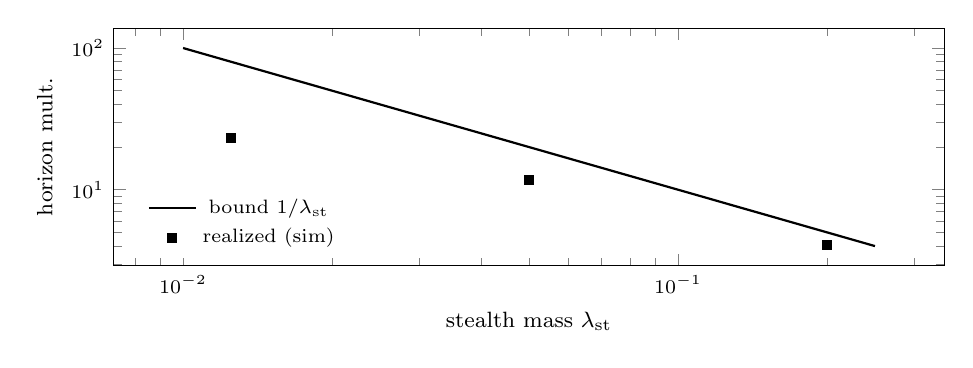
\begin{tikzpicture}
\begin{loglogaxis}[width=\textwidth,height=4.6cm,
  xlabel={stealth mass $\lst$},ylabel={horizon mult.},
  legend pos=south west,legend style={font=\scriptsize,draw=none},
  tick label style={font=\scriptsize},label style={font=\footnotesize}]
\addplot[no marks,thick,domain=0.01:0.25]{1/x};
\addplot[only marks,mark=square*,mark size=1.6pt]
  coordinates {(0.2,4.1)(0.05,11.8)(0.0125,23)};
\legend{bound $1/\lst$,realized (sim)}
\end{loglogaxis}
\end{tikzpicture}\\[-2pt]
{\scriptsize (b) Thm.~\ref{thm:ceiling}: realized gain under the $1/\lst$ ceiling.}
\end{minipage}
\caption{Simulation validation.
(a) The gate budget for fixed end-to-end reliability scales
linearly in $\log T$, the logarithmic-overhead regime;
the overhead axis is scaled by the
arbitrary per-gate cost ratio $g/s=0.2$, so only its slope, not its absolute height, is fixed
by the model.
(b) As the stealth floor falls, the realized
horizon multiplier rises toward---and stays under---the $1/\lst$ ceiling bound of
Theorem~\ref{thm:ceiling}.}
\label{fig:val}
\end{figure}

\section{Design implications}\label{sec:design}
Each is a falsifiable engineering claim.
\begin{enumerate}[leftmargin=1.6em,itemsep=3pt]
\item \textbf{Vote; do not require unanimity.} Under unanimity the false-reject rate grows as
$1-(1-\beta)^m$, so $\Padv$ falls geometrically and expected recomputation cost grows polynomially
in $T$.
Majority voting is what makes overhead logarithmic.
\item \textbf{Reset context on rollback.} Restoring the artifact but retaining a polluted working
context violates Assumption~\ref{a2} and reintroduces correlated failure: a naive rollback that
keeps the conversation history active forces the agent to resample from an error-polluted prior,
so successive retries are no longer independent.
The clean-context
rollback is what makes the memoryless model hold.
\item \textbf{Spend on diversity, not depth.} Beyond a computable per-family depth, additional
same-family gates do not lower the ceiling (Thm.~\ref{thm:ceiling});
budget belongs in independent
modalities, including at least one grounded in execution against the real environment, which alone
reduces the irreducible component $\lirr$ of the stealth mass (Prop.~\ref{prop:decomp}).
\item \textbf{Compute the checkpoint interval.} $s^\star=\sqrt{G/\lambda}$ with $\lambda$ estimated
from the agent's measured half-life and $G$ from the gate stack's latency.
\end{enumerate}

\section{The cost of a gate}\label{sec:gatecost}
The per-gate cost $g$ appears in neither ceiling: it scales the fixed-$s$ overhead
$(1+(g/s)\,m)/\Padv$ and, through
$G=mg$, the optimal interval $s^\star=\sqrt{G/\lambda}$ and the minimal overhead
$1+2\sqrt{mg\lambda}$ (Thm.~\ref{thm:interval}), but it cannot move the reliable horizon, which
Theorem~\ref{thm:ceiling} and Proposition~\ref{prop:decomp} set by stealth mass alone.
Our
simulation accordingly treats $g$ as a free scale and we fix it arbitrarily (\S\ref{sec:simulation}).
A real verification stack is not so free: each modality carries its own $g$, and---this is the
operative tension---cost and coverage are coupled.

\paragraph{Fast gates are what we want.} Every result in the threshold regime rewards low $g$.
Logarithmic overhead (Thm.~\ref{thm:threshold}) comes from stacking $m=O(\log T)$ gates per
checkpoint, and the constant multiplying that logarithm is exactly $g/s$.
Cheap gates let depth
grow with the horizon at negligible cost, let diversity (Cor.~\ref{cor:diversity}) be bought in
breadth rather than rationed, and---via $s^\star=\sqrt{G/\lambda}$---permit short checkpoint
intervals that localize faults tightly.
A system whose gates are nearly free can be verified
almost arbitrarily hard; the entire engineering pressure is toward driving $g$ down.
Table~\ref{tab:gatecost} makes the magnitude concrete: holding the gate counts at the
Fig.~\ref{fig:val}a values, a fast gate ($g/s=0.04$) verifies the $T=10^5$ horizon at $8\times$
overhead where a very slow one ($g/s=2$) costs $338\times$---a $\sim\!40\times$ spread at identical
reliability and identical $m$, since $g$ moves only the height.
Retuning the checkpoint interval to
the cost-optimal $s^\star$ (Thm.~\ref{thm:interval}) absorbs most but not all of the penalty (the
$338\times$ falls to $17\times$), at the price of coarser fault localization.

\begin{table}[t]
\centering
\small
\begin{tabular}{lccccc}
\toprule
 & & \multicolumn{3}{c}{overhead, fixed $s=0.25$} & opt.\ $s^\star$ \\
\cmidrule(lr){3-5}\cmidrule(lr){6-6}
gate cost $g$ & $g/s$ & $T{=}10$ & $T{=}10^3$ & $T{=}10^5$ & $T{=}10^5$ \\
\midrule
$0.01$ (fast)      & $0.04$ & $3.0$  & $5.4$   & $8.0$   & $3.3$  \\
$0.05$ (baseline)  & $0.20$ & $9.7$  & $22.1$  & $34.9$  & $6.1$  \\
$0.20$ (slow)      & $0.80$ & $35.1$ & $84.5$  & $135.8$ & $11.2$ \\
$0.50$ (very slow) & $2.00$ & $85.8$ & $209.3$ & $337.7$ & $17.2$ \\
\bottomrule
\end{tabular}
\caption{Overhead multiplier versus per-gate cost $g$, with the gate counts held at the
Fig.~\ref{fig:val}a values ($m=33,57,81,105,131$ for $T=10,\dots,10^5$): $g$ rescales overhead but
not $m$. Overhead is expected time per accepted segment, including recomputation of rejected
segments (the $1/\Padv$ factor). The last column retunes the checkpoint interval to the
cost-optimal $s^\star$ (Thm.~\ref{thm:interval}), which softens---but does not erase---the cost of
slow gates.}
\label{tab:gatecost}
\end{table}

\paragraph{But the gates we can make fast are not the gates that raise the ceiling.} The
difficulty is that $g$ is empirically correlated with the property that actually matters---a
gate's power to reduce the irreducible stealth mass $\lirr$ (Prop.~\ref{prop:decomp}). The cheap,
fast modalities tend to be the shallow ones.
\begin{itemize}[leftmargin=1.4em,itemsep=2pt]
\item \textbf{Unit and regression tests} (low $g$): milliseconds to run, fully automatable, the
natural depth dimension. But a test checks only the behavior it encodes, and a suite written from
the same specification as the agent inherits that specification's blind spots. Tests buy depth
cheaply and move $\lirr$ little.
\item \textbf{Knowledge-base / retrieval comparison} (low--medium $g$): checking an artifact
against a store of known-good references or documented constraints is fast and partly independent
of the generator, so it removes lineage-correlated mass $\lred$ the store does not share---but it
is blind wherever store and agent inherit the same error.
\item \textbf{Model-based review / LLM judge} (medium $g$): broad and flexible, but a judge sharing
a base model with the generator shares its blind spot ($\am$ correlated, $\lst$ unmoved). This is
a same-family gate, and depth within it plateaus at the family's stealth mass.
\item \textbf{Formal verification} (high $g$): for the properties it can express it drives the
false-accept rate toward zero and genuinely lowers $\lirr$ there---but it is slow, demands a formal
specification, and that specification is itself a source of $\lirr$ where it diverges from intent.
\item \textbf{Execution against the real environment} (high $g$): grounding---running the artifact
against the true system rather than a proxy---is the one modality the decomposition singles out as
able to reduce $\lirr$ (Rem.~\ref{rem:decomp}), because reality is the only oracle not derived from
the shared specification. It is also typically the most expensive gate: sandboxes, integration
environments, side effects, latency.
\end{itemize}
The pattern runs the wrong way: low $g$ correlates with shallow coverage (depth, which only helps
\emph{below} the ceiling), while ceiling-raising power ($\lirr$ reduction) correlates with high
$g$. The free-scale assumption of the simulation is therefore optimistic; a faithful cost model
would couple $g$ to a gate's position in the decomposition.

\paragraph{Where the leverage is.} This reframes the target. Depth is cheap but bounded---it cannot
cross the ceiling---whereas floor reduction is expensive but unbounded in value, so the
highest-return work is \emph{making the floor-reducing gates fast}: lowering $g$ for grounded
execution and formal checks rather than adding more of the cheap gates that have already saturated
their family.
Concretely: fast sandboxed execution with snapshotting to amortize environment setup;
incremental, compositional formal methods that verify a segment without re-verifying its past;
cached and indexed knowledge-base comparison; and property-based test generation that widens
coverage without hand-written cases.
Each is an attack on $g$ for a modality that moves $\lirr$.
Theorem~\ref{thm:ceiling} says how much such work is worth; the cost of the gate says whether it is
affordable; and progress on autonomous horizon is the joint optimization of the two. At present the
binding term is the cost of the gates that actually see.

\section{Proposed Experiment}\label{sec:experiment}
Run an agentic task suite with task-length labels under three conditions: (a) raw agents;
(b) checkpoint-gated agents with same-family stacks of increasing depth; (c) checkpoint-gated
agents with cross-family plus execution-grounded stacks.
The model predicts: (a) reproduces an
exponential success-decay baseline; (b) improves then plateaus at the independently-measured family
stealth mass $\lst$;
(c) shifts the horizon by $\approx 1/\lirr$ and, with depth scaled as
$\log T$, shows no plateau within budget.
A clean plateau in (b) at the measured $\lst$ would
confirm the ceiling;
horizon in (c) tracking model scale rather than gate diversity would falsify
the central claim.

\section{Limitations}\label{sec:limitations}
\paragraph{Modeled, not measured.} Every quantitative result in this paper is analytical or
in-simulation; we have not run the checkpoint-and-gate protocol on a deployed agentic system.
The empirical work we cite~\cite{ron2026} establishes that the stealth-mass regime is real for
code generators, not that this architecture attains the predicted horizons in practice.
The
experiment of \S\ref{sec:experiment} is precisely the test that would confirm or falsify this; we
therefore present the theory as a set of falsifiable predictions rather than validated engineering.
\paragraph{Checkpoint completeness (Assumption~\ref{a1}).} Gates check a machine-checkable proxy,
not intent; faults that satisfy the proxy but violate intent ride through every checkpoint and are
accounted within $\lst$---specifically within $\lirr$ (Prop.~\ref{prop:decomp}).
The ceiling
theorem therefore prices the specification gap rather than escaping it, and improvements to the
specification (moving fault mass out of $\lirr$) are the only lever the theorem does not already
capture.
Such intent-violating faults are systematically reproduced on retry, but this does not breach
Assumption~\ref{a2}: a stealthy fault passes every gate unanimously and so advances \emph{without}
recomputation, so the memoryless-retry model is never exercised on it.
These faults are \emph{absorbing}---once present they are never repaired---which is precisely why
they set a ceiling rather than being retried away.
\paragraph{Memorylessness (Assumption~\ref{a2}).} Real agents exhibit context poisoning, drift,
and error snowballing, which induce inter-segment correlation.
The clean-context rollback
(\S\ref{sec:design}) is a design measure to approximate the assumption; residual correlation
degrades the bounds toward the ceiling regime.
\paragraph{Benign executors.} The analysis governs incompetence, not malice. Against an adversary
who knows the protocol, recomputation aids the attacker (slip probability $1-(1-p_{\mathrm{evade}})^k$
grows with retries), and the threshold analysis requires a game-theoretic treatment that we leave
to future work~\cite{greenblatt2024}.
\paragraph{Constant hazard.} Real tasks have difficulty structure; a heterogeneous-hazard model
would refine the per-segment analysis and is the natural next step.
A clustered or time-varying
hazard---e.g.\ a burst of correlated errors during a single hard architectural step---leaves the
\emph{mean} checkpointing overhead governed by the same $\lambda$ but inflates its \emph{variance},
since bad segments then arrive in runs that trigger consecutive recomputations.
The constant-hazard
model is thus the necessary baseline that isolates the threshold phenomenon, with a time-varying
$\lambda(t)$ the natural refinement.

\section{Related work}\label{sec:related}
Reliable computation from unreliable components originates with von Neumann~\cite{vonneumann1956}
and Moore--Shannon~\cite{moore1956};
the fault-tolerance threshold for quantum computation is due
to~\cite{aharonov1997} and contemporaries.
Majority aggregation of noisy judgments is Condorcet's
jury theorem~\cite{condorcet1785}, with the correlated-voter correction due to~\cite{ladha1992}.
The cost-optimal checkpoint interval is Young's~\cite{young1974} and Daly's~\cite{daly2006}.

Our gate stack is the verification dual of classical $N$-version programming, proposed by Chen and
Avi\v{z}ienis~\cite{avizienis1978} and modeled by Avi\v{z}ienis~\cite{avizienis1985}: the
exponential-in-$N$ reliability of that model is the $\lst=0$ case of
Theorem~\ref{thm:threshold}, and its known failure---fault correlation---is our
Theorem~\ref{thm:ceiling}.
That independence cannot be assumed was shown theoretically by Eckhardt
and Lee~\cite{eckhardt1985} and Littlewood and Miller~\cite{littlewood1989}, and empirically by
Knight and Leveson~\cite{knight1986,brilliant1990}, with specification weakness identified as a
driver by Bishop~\cite{bishop1988} and useful reliability gains despite correlation observed by
Hatton~\cite{hatton1997}.
Ron, Baudry, and Monperrus~\cite{ron2026} reproduce the
Knight--Leveson experiment with contemporary coding agents and find the same correlated-failure
structure, supplying the empirical warrant for our bounded regime.
Our contribution relative to
this line is twofold: we place agentic long-horizon reliability within the classical
fault-tolerance-threshold framework, obtaining logarithmic overhead and a closed-form checkpoint
interval rather than a fixed-$N$ vote;
and we decompose the correlation floor
(Prop.~\ref{prop:decomp}) into a diversity-reducible part and a specification-bound irreducible
part, separating a priori what diversity can and cannot fix.
On the agentic side, the horizon metric and its growth are reported by~\cite{metr2025}, with the
constant-hazard reading in~\cite{ord2025};
verification-centric inference scaling and its
non-monotonicities appear in~\cite{brown2024}; and the adversarial regime is studied under the
heading of AI control in~\cite{greenblatt2024}.

\section{Conclusion}
Within a standard constant-hazard model, the reliable horizon of an agentic system is governed
above a threshold not by the agent's raw error rate but by the shared blind-spot mass of its
verification stack, with the horizon multiplier bounded by its reciprocal---and, once that mass is
decomposed, by the reciprocal of its specification-bound part alone.
Because the reducible mass is
measurable from a system's own logs and is reduced by verification diversity rather than depth, a
substantial share of long-horizon reliability is available as verification engineering today,
independent of further gains in model capability.
In practice this reduces to two architectural rules: reset the agent's context on every rollback,
so retries stay independent (Assumption~\ref{a2}); and spend verification budget on diverse
modalities---different model lineages, test types, and at least one grounded in execution against
the real environment---rather than on more gates of the same family.

\section*{Code and data availability}
All code reproducing the results of \S\ref{sec:simulation}---and the complete listing of
Appendix~\ref{app:code}---is available at \url{https://github.com/ivmat/gated-computation-sim} and
archived on Zenodo (DOI: \href{https://doi.org/10.5281/zenodo.20820968}{10.5281/zenodo.20820968}).

\begin{thebibliography}{99}
\small
\bibitem{vonneumann1956} J.~von Neumann. Probabilistic logics and the synthesis of reliable
organisms from unreliable components.
In \emph{Automata Studies}, Princeton Univ.\ Press, 1956.
\bibitem{moore1956} E.~F.~Moore and C.~E.~Shannon. Reliable circuits using less reliable relays.
\emph{J.~Franklin Inst.}, 1956.
\bibitem{aharonov1997} D.~Aharonov and M.~Ben-Or. Fault-tolerant quantum computation with constant
error. In \emph{STOC}, 1997.
\bibitem{condorcet1785} M.~de Condorcet.
\emph{Essai sur l'application de l'analyse \`a la
probabilit\'e des d\'ecisions rendues \`a la pluralit\'e des voix.} 1785.
\bibitem{ladha1992} K.~K.~Ladha.
The Condorcet jury theorem, free speech, and correlated votes.
\emph{Amer.\ J.\ Political Science}, 1992.
\bibitem{young1974} J.~W.~Young.
A first order approximation to the optimum checkpoint interval.
\emph{Comm.\ ACM}, 1974.
\bibitem{daly2006} J.~T.~Daly.
A higher order estimate of the optimum checkpoint interval for
restart dumps.
\emph{Future Generation Computer Systems}, 2006.
% --- N-version programming lineage ---
\bibitem{avizienis1978} L.~Chen and A.~Avi\v{z}ienis.
On the implementation of $N$-version
programming for software fault tolerance during execution. In \emph{COMPSAC}, 1977--78.
\bibitem{avizienis1985} A.~Avi\v{z}ienis.
The $N$-version approach to fault-tolerant software.
\emph{IEEE Trans.\ Software Eng.}, 1985.
\bibitem{eckhardt1985} D.~E.~Eckhardt and L.~D.~Lee.
A theoretical basis for the analysis of
multiversion software subject to coincident errors. \emph{IEEE Trans.\ Software Eng.}, 1985.
\bibitem{littlewood1989} B.~Littlewood and D.~Miller.
Conceptual modeling of coincident failures
in multiversion software. \emph{IEEE Trans.\ Software Eng.}, 1989.
\bibitem{knight1986} J.~C.~Knight and N.~G.~Leveson.
An experimental evaluation of the assumption
of independence in multiversion programming. \emph{IEEE Trans.\ Software Eng.}, 1986.
\bibitem{brilliant1990} S.~S.~Brilliant, J.~C.~Knight, and N.~G.~Leveson.
Analysis of faults in an
$N$-version software experiment. \emph{IEEE Trans.\ Software Eng.}, 1990.
\bibitem{bishop1988} P.~G.~Bishop.
The PODS diversity experiment.
In U.~Voges (Ed.), \emph{Software Diversity in Computerized Control Systems}, Springer, 1988,
pp.~51--84.
\bibitem{hatton1997} L.~Hatton. N-version design versus one good version.
\emph{IEEE Software},
1997.
\bibitem{ron2026} J.~Ron, B.~Baudry, and M.~Monperrus. N-Version Programming with Coding Agents.
\emph{arXiv:2606.20158}, 2026.
% --- agentic side ---
\bibitem{metr2025} T.~Kwa, B.~West, et al.\ (METR). Measuring AI Ability to Complete Long
Tasks.
\emph{arXiv:2503.14499}, 2025.
\bibitem{ord2025} T.~Ord. Is there a Half-Life for the Success Rates of AI Agents?
Online essay, \url{https://tobyord.com/writing/half-life}, 2025.
\bibitem{brown2024} B.~Brown, J.~Juravsky, R.~Ehrlich, R.~Clark, Q.~V.~Le, C.~R\'e, and A.~Mirhoseini. Large Language Monkeys: Scaling inference compute
with repeated sampling.
\emph{arXiv:2407.21787}, 2024.
\bibitem{greenblatt2024} R.~Greenblatt, B.~Shlegeris, K.~Sachan, and F.~Roger. AI Control: Improving safety despite
intentional subversion. In \emph{Proceedings of the 41st International Conference on Machine Learning (ICML)}, 2024.
\end{thebibliography}

\appendix
\section{Simulation code}\label{app:code}
The complete, self-contained script below reproduces every numerical result of
\S\ref{sec:simulation}---the threshold and ceiling figures (Figure~\ref{fig:val}), the
per-segment-slip check, the optimal-interval scan, the three-arm diversity comparison, and the
gate-cost sweep of Table~\ref{tab:gatecost}---computed by the functions \texttt{experiment1},
\texttt{experiment2}, \texttt{experiment\_slip}, \texttt{experiment\_interval},
\texttt{experiment\_threearm}, and \texttt{gate\_cost\_sweep}.
It keeps the exact
discrete-event model but collapses each segment's geometric recomputation loop to its marginal slip
probability $\eseg=p\,\am/\Padv$ (Lemma~\ref{lem:slip}); with independent segments end-to-end
success is exactly $(1-\eseg)^n$, which the experiments evaluate directly (so the reported numbers
are seed-independent), with $\am,\bm$ exact binomial majority-tails.
The routine
\texttt{validate\_against\_original} runs the literal slow discrete-event simulation---success
over $\mathrm{Binomial}(n,\eseg)$ trials---and checks it matches the closed form within sampling
noise before any figure is produced.
As noted in
\S\ref{sec:simulation}, the per-gate cost \texttt{G\_PER\_GATE}~$=g$ is arbitrary and enters only
as the ratio $g/s$ that scales the overhead axis of Fig.~\ref{fig:val}a.

\begin{lstlisting}[language=Python]
"""
Vectorized, validated reproduction of simulate_n1.py (Fig 1a/1b).

Why this file exists
--------------------
The original pure-Python loop cannot reach the paper's Fig 1a horizon (T=1e5):
it needs a majority stack of m~=127 gates there, which is ~1e10 segment
evaluations (~16 h) AND it crashes, because for T>=100 no m<=49 ever reaches
90% success so the `overheads` list ends up shorter than `horizons`.

This file keeps the EXACT model but exploits two facts:
  (1) Experiment-1 overhead is deterministic given m. The original loop reassigned
      `time_spent = s + G` each round, undercounting recomputation; we use the
      correct expected time per accepted segment, (s+G)/Padv, so
      overhead = (1 + (g/s)m)/Padv -- the 1/Padv counts recomputation of rejected
      segments (Lemma 1).
  (2) Per segment, P(slip) = eseg = p*am_bar/Padv (Lemma 1), and segments are
      independent, so end-to-end success is exactly (1-eseg)^n. am_bar, bm are
      EXACT binomial majority-tails, so no approximation enters.

The experiments evaluate these closed forms directly, so the reported numbers
are seed-independent. validate_against_original() runs the literal slow
discrete-event Monte Carlo -- success over Binomial(n, eseg) trials -- and
checks it matches the closed form within sampling noise before any results are
trusted.
"""
import numpy as np
import matplotlib.pyplot as plt
from math import comb

# Per-gate evaluation time g.
# NOTE: g is an ARBITRARY illustrative constant -- we have no empirical value
# for it. It enters the results ONLY through the ratio g/s, which sets the
# VERTICAL SCALE of Fig 1a via  overhead = (1 + (g/s)*m)/Padv. It changes neither the
# required gate counts m (Fig 1a x-shape), nor the horizon ceiling (Fig 1b),
# nor any theorem; the log-linear growth and its ~ln10/(2*(1/2-alpha)^2) slope
# (Remark 1) are invariant to g. We fix g = 0.05, giving g/s = 0.2 at s = 0.25.
G_PER_GATE = 0.05


# ----------------------------------------------------------------------
# ORIGINAL slow model (verbatim) -- kept ONLY to validate the slip/success
# statistics (eseg and end-to-end success) against the fast closed form.
# It still carries the old timing undercount (time_spent is reassigned each
# round, so it omits the 1/Padv recomputation factor); it is therefore NOT a
# valid source of overhead/timing numbers -- those come from overhead_for_m().
# ----------------------------------------------------------------------
def run_segment_recomputation(s, lam, m, alpha, beta, lst):
    g = G_PER_GATE
    Gtot = m * g
    while True:
        p_fault = 1.0 - np.exp(-lam * s)
        has_fault = np.random.rand() < p_fault
        if has_fault:
            is_stealthy = np.random.rand() < lst
            if is_stealthy:
                passed = True
            else:
                votes_accept = np.random.rand(m) < alpha
                passed = np.sum(votes_accept) > (m / 2)
        else:
            votes_reject = np.random.rand(m) < beta
            failed = np.sum(votes_reject) > (m / 2)
            passed = not failed
        time_spent = s + Gtot
        if passed:
            return time_spent, has_fault


def simulate_horizon_slow(T, s, lam, m, alpha, beta, lst):
    n_segments = int(np.ceil(T / s))
    total_time = 0
    successful = True
    for _ in range(n_segments):
        time_spent, slipped = run_segment_recomputation(s, lam, m, alpha, beta, lst)
        total_time += time_spent
        if slipped:
            successful = False
    return successful, total_time


# ----------------------------------------------------------------------
# FAST model -- exact same statistics, vectorized
# ----------------------------------------------------------------------
def majority_tail(m, q):
    """Exact P[Binom(m, q) > m/2] (the original's `sum(votes) > m/2`)."""
    kmin = m // 2 + 1
    return float(sum(comb(m, k) * q**k * (1.0 - q) ** (m - k) for k in range(kmin, m + 1)))


def advance_prob(s, lam, m, alpha, beta, lst):
    """Padv: probability the recomputation loop advances in a given round (Lemma 1)."""
    p = 1.0 - np.exp(-lam * s)
    am_bar = lst + (1.0 - lst) * majority_tail(m, alpha)   # P(pass | bad), stealth mixture
    bm = majority_tail(m, beta)                            # P(fail | good)
    return (1.0 - p) * (1.0 - bm) + p * am_bar


def segment_slip_prob(s, lam, m, alpha, beta, lst):
    """eseg = p*am_bar/Padv  (Lemma 1), with am_bar, bm exact binomial tails."""
    p = 1.0 - np.exp(-lam * s)
    am_bar = lst + (1.0 - lst) * majority_tail(m, alpha)
    return p * am_bar / advance_prob(s, lam, m, alpha, beta, lst)


def success_rate_fast(T, s, lam, m, alpha, beta, lst, trials, rng):
    """Monte-Carlo end-to-end success rate over `trials` runs (vectorized)."""
    n = int(np.ceil(T / s))
    eseg = segment_slip_prob(s, lam, m, alpha, beta, lst)
    slips = rng.binomial(n, eseg, size=trials)   # #slips per trial
    return float(np.mean(slips == 0))


def overhead_for_m(T, s, m, padv):
    """Expected time per accepted segment / useful work, INCLUDING recomputation of
    rejected segments: (1 + (g/s)*m) / Padv. The 1/Padv factor is the expected number
    of recomputation rounds per accepted segment (Lemma 1 / Thm 1); the original loop
    omitted it by reassigning time_spent each round, undercounting overhead by
    ~1/Padv ~ e^{lam*s}."""
    n = int(np.ceil(T / s))
    return n * (s + m * G_PER_GATE) / T / padv


# ----------------------------------------------------------------------
# VALIDATION: fast vs original slow, on small cases
# ----------------------------------------------------------------------
def validate_against_original():
    print("=" * 64)
    print("VALIDATION: fast success-rate vs original slow simulate_horizon")
    print("=" * 64)
    s, lam, alpha, beta = 0.25, 1.0, 0.3, 0.1
    rng = np.random.default_rng(0)
    ok = True
    cases = [
        # (T, m, lst)
        (10, 5, 0.0), (10, 15, 0.0), (10, 29, 0.0),
        (5, 21, 0.20), (8, 21, 0.05),
    ]
    for (T, m, lst) in cases:
        trials = 4000
        # slow (original) empirical success rate
        np.random.seed(12345)
        slow = np.mean([simulate_horizon_slow(T, s, lam, m, alpha, beta, lst)[0]
                        for _ in range(trials)])
        fast = success_rate_fast(T, s, lam, m, alpha, beta, lst, trials, rng)
        # binomial sampling noise ~ sqrt(p(1-p)/trials) <= 0.008; allow 4 sigma
        tol = 4.0 * np.sqrt(0.25 / trials) + 0.005
        good = abs(slow - fast) <= tol
        ok = ok and good
        print(f"  T={T:>3} m={m:>3} lst={lst:<6}  slow={slow:.4f}  fast={fast:.4f}"
              f"  |d|={abs(slow-fast):.4f}  tol={tol:.4f}  {'OK' if good else 'MISMATCH'}")
    print(f"VALIDATION {'PASSED' if ok else 'FAILED'}\n")
    return ok


# ----------------------------------------------------------------------
# EXPERIMENT 1: threshold & logarithmic overhead (to T = 1e5)
# ----------------------------------------------------------------------
def experiment1():
    print("Running Experiment 1 (Logarithmic Overhead vs Log T)  [to T=1e5]...")
    s, lam, alpha, beta = 0.25, 1.0, 0.3, 0.1
    horizons = [10, 100, 1000, 10000, 100000]
    m_ceiling = 301                       # raised from 51 -> reaches 1e5
    # Smallest odd m whose EXACT end-to-end success (1-eseg)^n >= 0.90. The
    # discrete-event Monte Carlo behind eseg is checked in
    # validate_against_original(); evaluating the validated model directly makes
    # the reported gate counts seed-independent (a 500-trial search was noisy at
    # small T, returning m off by one step).
    req_m, overheads, solved_T = [], [], []
    for T in horizons:
        n = int(np.ceil(T / s))
        for m in range(1, m_ceiling, 2):
            if (1.0 - segment_slip_prob(s, lam, m, alpha, beta, 0.0)) ** n >= 0.90:
                req_m.append(m)
                overheads.append(overhead_for_m(T, s, m, advance_prob(s, lam, m, alpha, beta, 0.0)))
                solved_T.append(T)
                break
        else:
            print(f"  WARNING: no m < {m_ceiling} reached 90% for T={T}")
    print("  log10 T :", [round(np.log10(t), 1) for t in solved_T])
    print("  req. m  :", req_m)
    print("  overhead:", [round(o, 2) for o in overheads])
    return solved_T, req_m, overheads


# ----------------------------------------------------------------------
# EXPERIMENT 2: horizon ceiling vs stealth mass
# ----------------------------------------------------------------------
def experiment2():
    print("Running Experiment 2 (Horizon Ceiling vs Stealth Mass)...")
    s, lam, alpha, beta, m = 0.25, 1.0, 0.3, 0.1, 21
    stealth_masses = [0.20, 0.05, 0.0125]
    bounds = [1.0 / x for x in stealth_masses]
    H_raw = np.log(2) / lam
    # Exact 50% horizon of the validated model: success(T)=(1-eseg)^(T/s)=0.5,
    # so T50 = s*ln(0.5)/ln(1-eseg). Avoids the grid quantization of a search.
    realized = []
    for lst in stealth_masses:
        eseg = segment_slip_prob(s, lam, m, alpha, beta, lst)
        T50 = s * np.log(0.5) / np.log(1.0 - eseg)
        realized.append(T50 / H_raw)
    print("  stealth mass   :", stealth_masses)
    print("  bound 1/lst    :", [round(b, 1) for b in bounds])
    print("  realized mult. :", [round(r, 1) for r in realized])
    return stealth_masses, bounds, realized


# ----------------------------------------------------------------------
# --- GATE-COST SWEEP: overhead vs horizon for several per-gate costs g ---
# g does NOT change the required gate counts m (those are set by alpha/beta/lst),
# so we reuse experiment1's m and rescale: overhead(T,g) = 1 + (g/s)*m at fixed
# s=0.25 (the Fig 1a protocol). We also report the cost-optimal overhead
# 1 + 2*sqrt(m*g*lam) reachable if the checkpoint interval is retuned (Thm 3).
def gate_cost_sweep(solved_T, req_m, s=0.25, lam=1.0, alpha=0.3, beta=0.1,
                    g_values=(0.01, 0.05, 0.2, 0.5)):
    labels = {0.01: "fast", 0.05: "baseline", 0.2: "slow", 0.5: "very slow"}
    print("\nGate-cost sweep (overhead at fixed s=0.25):")
    header = "  log10T  " + "".join(f"g={g:<5}({labels.get(g,''):<9})" for g in g_values)
    print(header)
    padv = [advance_prob(s, lam, m, alpha, beta, 0.0) for m in req_m]
    fixed = {g: [(1.0 + (g / s) * m) / pv for m, pv in zip(req_m, padv)] for g in g_values}
    optimal = {g: [1.0 + 2.0 * np.sqrt(m * g * lam) for m in req_m] for g in g_values}
    for i, T in enumerate(solved_T):
        row = f"  {np.log10(T):>5.0f}   "
        row += "".join(f"{fixed[g][i]:>7.1f}        " for g in g_values)
        print(row)
    print("  (cost-optimal s*, same m):")
    for i, T in enumerate(solved_T):
        row = f"  {np.log10(T):>5.0f}   "
        row += "".join(f"{optimal[g][i]:>7.1f}        " for g in g_values)
        print(row)

    plt.figure(figsize=(6, 4))
    for g in g_values:
        plt.plot(np.log10(solved_T), fixed[g], 'o-',
                 label=f"g={g} (g/s={g/s:.2f}, {labels.get(g,'')})")
    plt.yscale('log')
    plt.xlabel(r'$\log_{10} T$')
    plt.ylabel(r'Overhead Multiplier ($\times$), fixed $s=0.25$')
    plt.title('Overhead vs horizon for different per-gate costs $g$')
    plt.grid(True, which='both', linestyle=':', alpha=0.6)
    plt.legend(fontsize=8)
    plt.tight_layout()
    plt.savefig('gate_cost_overhead.png', dpi=300)
    return fixed, optimal


# ----------------------------------------------------------------------
# PER-SEGMENT SLIP (Lemma 1): closed-form eseg vs discrete-event Monte Carlo
# ----------------------------------------------------------------------
def experiment_slip(m=5, trials=20000, seed=2024):
    s, lam, alpha, beta = 0.25, 1.0, 0.3, 0.1
    predicted = segment_slip_prob(s, lam, m, alpha, beta, 0.0)
    np.random.seed(seed)
    slips = [run_segment_recomputation(s, lam, m, alpha, beta, 0.0)[1] for _ in range(trials)]
    mc = float(np.mean(slips))
    print(f"Per-segment slip (Lemma 1, m={m}): predicted eseg={predicted:.4f}  "
          f"Monte-Carlo={mc:.4f}  ({trials} trials)")
    return predicted, mc


# ----------------------------------------------------------------------
# OPTIMAL CHECKPOINT INTERVAL (Theorem 3)
# C(s) = (1+G/s) e^{lam s} / (1-bm); compare numerical argmin to s*=sqrt(G/lam).
# ----------------------------------------------------------------------
def experiment_interval(m=5):
    s_dummy, lam, alpha, beta = 0.25, 1.0, 0.3, 0.1
    G = m * G_PER_GATE
    bm = majority_tail(m, beta)
    grid = np.linspace(0.02, 2.0, 4000)
    cost = (1.0 + G / grid) * np.exp(lam * grid) / (1.0 - bm)
    s_num = float(grid[np.argmin(cost)])
    s_pred = float(np.sqrt(G / lam))
    foc = (-G + np.sqrt(G * G + 4.0 * G / lam)) / 2.0   # exact root of s(s+G)=G/lam
    ov_num = float(np.min(cost))
    ov_pred = 1.0 + 2.0 * np.sqrt(G * lam)
    print(f"Optimal interval (Thm 3, m={m}, G={G:.3f}): s*=sqrt(G/lam)={s_pred:.3f}, "
          f"exact-FOC root={foc:.3f}, numerical argmin={s_num:.3f}; "
          f"min overhead={ov_num:.3f} (approx 1+2sqrt(G lam)={ov_pred:.3f})")
    return s_pred, s_num


# ----------------------------------------------------------------------
# THREE-ARM DIVERSITY COMPARISON (Cor. 1 / Prop. 1)
# raw vs same-family depth vs independent diverse families, equal gate budget.
# ----------------------------------------------------------------------
def stack_slip_prob(s, lam, families, alpha, beta):
    """eseg for a stack of INDEPENDENT gate families.
    families: list of (stealth_mass, depth) -- a segment must pass every family."""
    p = 1.0 - np.exp(-lam * s)
    pass_bad, pass_good = 1.0, 1.0
    for (lst_i, m_i) in families:
        pass_bad *= lst_i + (1.0 - lst_i) * majority_tail(m_i, alpha)
        pass_good *= 1.0 - majority_tail(m_i, beta)
    padv = (1.0 - p) * pass_good + p * pass_bad
    return p * pass_bad / padv


def experiment_threearm(budget=21, n_families=3, lst_fam=0.15):
    s, lam, alpha, beta = 0.25, 1.0, 0.3, 0.1
    H_raw = np.log(2) / lam

    def mult(families):
        eseg = stack_slip_prob(s, lam, families, alpha, beta)
        return s * np.log(0.5) / np.log(1.0 - eseg) / H_raw

    same = mult([(lst_fam, budget)])                              # one family, full depth
    depth = budget // n_families
    diverse = mult([(lst_fam, depth)] * n_families)               # k independent families
    # stealth mass recovered from the same-family arm's effective floor
    eseg_same = stack_slip_prob(s, lam, [(lst_fam, budget)], alpha, beta)
    am_bar_recovered = lst_fam + (1.0 - lst_fam) * majority_tail(budget, alpha)
    print(f"Three-arm (budget={budget} gates, lst_fam={lst_fam}): "
          f"raw=1.0x  same-family({budget})={same:.1f}x  "
          f"diverse({n_families}x{depth})={diverse:.1f}x  separation={diverse/same:.0f}x")
    print(f"  recovered same-family floor am_bar={am_bar_recovered:.3f} "
          f"(predicts ceiling ~{1.0/am_bar_recovered:.1f}x; realized {same:.1f}x)")
    return same, diverse


def main():
    if not validate_against_original():
        raise SystemExit("Fast model failed validation -- not plotting.")

    experiment_slip()
    solved_T, req_m, overheads = experiment1()
    stealth_masses, bounds, realized = experiment2()
    experiment_interval()
    experiment_threearm()
    gate_cost_sweep(solved_T, req_m)

    plt.figure(figsize=(10, 4))

    plt.subplot(1, 2, 1)
    plt.plot(np.log10(solved_T), overheads, 'o--', color='blue', label='Simulation')
    plt.xlabel(r'$\log_{10} T$')
    plt.ylabel(r'Overhead Multiplier ($\times$)')
    plt.title(r'(a) Logarithmic Overhead Regime ($\lambda_{st}=0$)')
    plt.grid(True, linestyle=':', alpha=0.6)
    plt.legend()

    plt.subplot(1, 2, 2)
    plt.loglog(stealth_masses, bounds, '-', color='black',
               label=r'Theoretical Bound ($1/\lambda_{st}$)')
    plt.loglog(stealth_masses, realized, 's', color='red', label='Realized Gated Horizon')
    plt.xlabel(r'Stealth Mass ($\lambda_{st}$)')
    plt.ylabel(r'Horizon Multiplier ($\times$)')
    plt.title('(b) Ceiling Scaling Bound')
    plt.grid(True, which="both", linestyle=':', alpha=0.6)
    plt.legend()

    plt.tight_layout()
    out = 'gated_computation_validation_FULL.png'
    plt.savefig(out, dpi=300)
    print(f"\nSimulation complete. Plots saved to '{out}'.")


if __name__ == "__main__":
    main()
\end{lstlisting}

\end{document}